 \item Rejestracja klienta \\
 
 Opis słowny - jest to pierwszy przypadek użycia dla klienta, bez którego
 pozostałe przypadki nie mają racji bytu. Akcje w nim opisane mają miejsce, gdy
 użytkownik pierwszy raz pojawia się na stronie i po przejrzeniu oferty sklepu
 (co dostępne jest także dla użytkowników niezalogowanych) decyduje się na
 stworzenie konta i ewentualne rozpoczęcie zakupów. Obsługa tego przypadku
 użycia wymaga poprawnego procesowania operacji rejestracji i jej potwierdzenia.
 
 \begin{longtable}{|p{5cm}|p{7cm}|}
 	\hline
	\textbf{Aktor} & Klient \\
	\hline
	\textbf{Warunki początkowe} & Klient niezalogowany, posiadający konto e-mail \\
	\hline
	\textbf{Opis przebiegu interakcji} & Wybór okna rejestracji, wypełnienie
	danych, potwierdzenia poprzez wiadomość e-mail \\
	\hline
	\textbf{Sytuacje wyjątkowe} & Klient już istniejący w bazie danych, brak konta
	e-mail \\
	\hline
	\textbf{Warunki końcowe} & Zarejestrowanie nowego klienta w systemie \\
	\hline
 \end{longtable}
 
  \item Rejestracja klienta - scenariusz główny \\
  \begin{tabularx}{\linewidth}{ c X}
  Aktor: & Klient \\
  \end{tabularx}
   \begin{enumerate}
    \item Klient uruchamia stronę internetową sklepu i wybiera opcję rejestracji
    \item Klient wstawia swoje dane osobowe i wybiera domyślny model płatności
    (kartą, za pobraniem itp.)
    \item System sprawdza wstawione dane (takie same hasła, czy istnieje już
    zarejestrowany w systemie użytkownik, czy istnieje podany adres e-mail itp.)
    \item System wysyła e-mail powitalny na adres podany przez klienta
    \item W ciągu określonego, zdefiniowanego czasu klient wybiera przesłany w
    e-mailu link, stając się pełnoprawnym użytkownikiem sklepu. Dane zapisywane
    są w bazie danych użytkowników a użytkownik może zalogować się  do systemu
  \end{enumerate}
  
  
  \item Rejestracja klienta - scenariusz alternatywny - klient już
  zarejestrowany w systemie \\
  \begin{tabularx}{\linewidth}{ c X}
  Aktor: & Klient \\
  \end{tabularx}
   \begin{enumerate}
     \item Kroki 1-2 scenariusza głównego
     \item System informuje użytkownika, że jest już zarejestrowany w systemie
     \item System przenosi użytkownika do ekranu logowania
   \end{enumerate} 
   
   \item Rejestracja klienta - scenariusz alternatywny - klient nie posiada
   adresu e-mail
   \begin{tabularx}{\linewidth}{ c X}
	Aktor: & Klient \\
  	\end{tabularx}   
  	\begin{enumerate}
  	  \item Kroki 1-4 scenariusza głównego
  	  \item System informuje użytkownika, że podany adres e-mail nie istnieje i
  	  przenosi użytkownika z powrotem do ekranu wypełniania danych wraz z
  	  adnotacją, by przed dalszą rejestracją założył konto e-mail.
  	\end{enumerate}
  	
  	
\item Rejestracja klienta - scenariusz alternatywny - klient nie klika w linka
aktywacyjny
   \begin{tabularx}{\linewidth}{ c X}
	Aktor: & Klient \\
  	\end{tabularx}   
  	\begin{enumerate}
  	  \item Kroki 1-5 scenariusza głównego
  	  \item System odrzuca prośbę użytkownika o rejestrację i nie umieszcza jego
  	  danych w bazie użytkowników. Przy następnym rozpoczęciu procesowania
  	  przypadku użycia Rejestracja Klienta klient musi od nowa wypełnić wszystkie
  	  dane. Do tego czasu nie może korzystać z opcji dostępnych tylko dla osób
  	  zalogowanych.
  	\end{enumerate}
  	
  	
  	
\begin{figure}[H]
    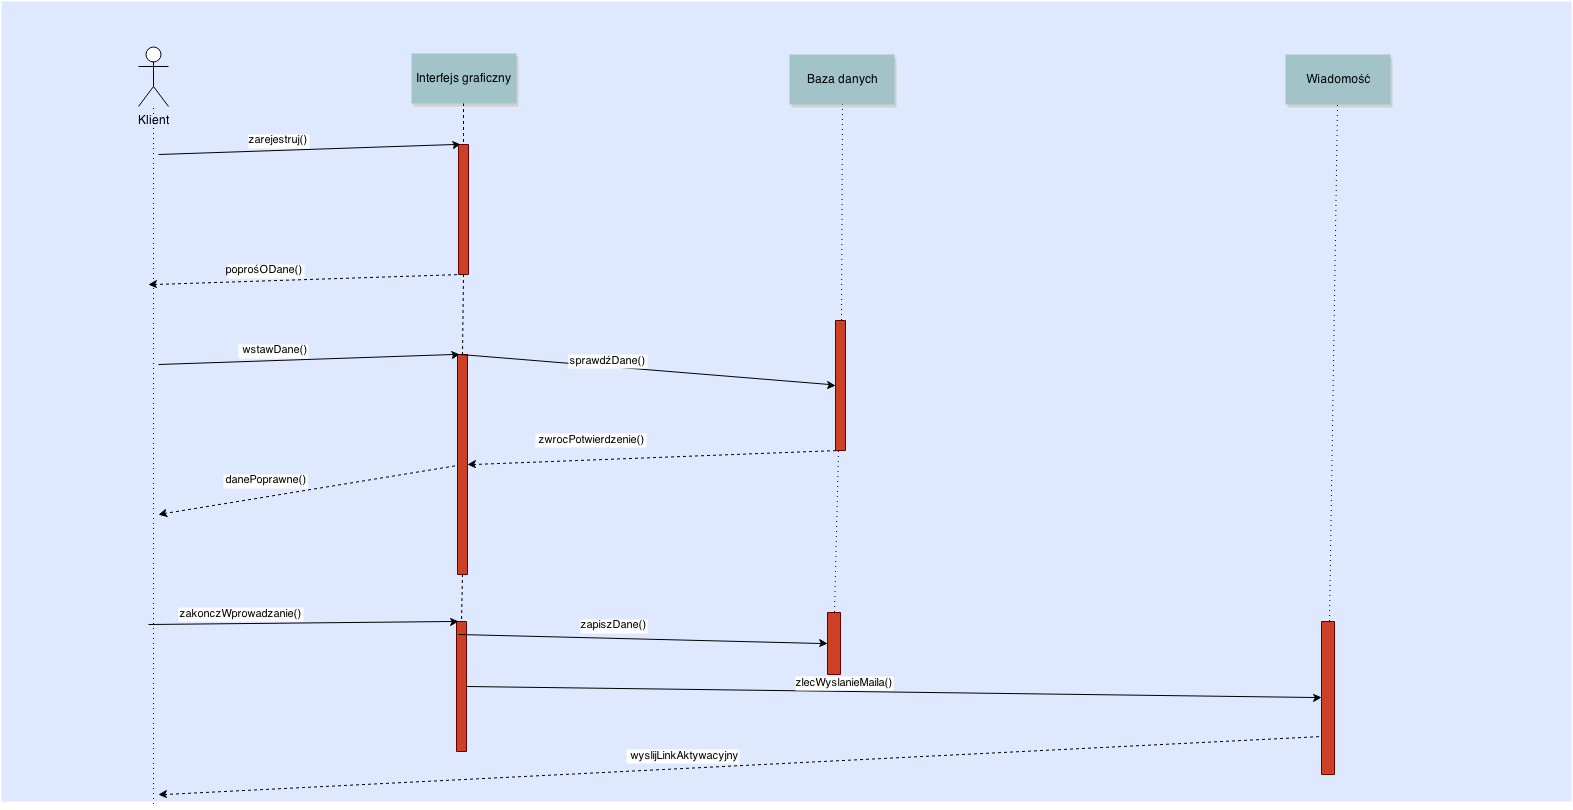
\includegraphics[width=\textwidth,
    height=0.5\textheight]{graphics/UseCase/Klient/RejestracjaKlientaSD.png}
  \caption{Diagram sekwencji dla przypadku użycia Rejestracja Klienta -
  scenariusz główny}
\end{figure}